\thispagestyle{lichsutoanhocnone}
\pagestyle{lichsutoanhoc}
\graphicspath{{../lichsutoanhoc/pic/}}
\everymath{\color{lichsutoanhoc}}
\blfootnote{$^1$\color{lichsutoanhoc}Cộng tác viên Viện Toán học.}
\begingroup
\AddToShipoutPicture*{\put(0,616){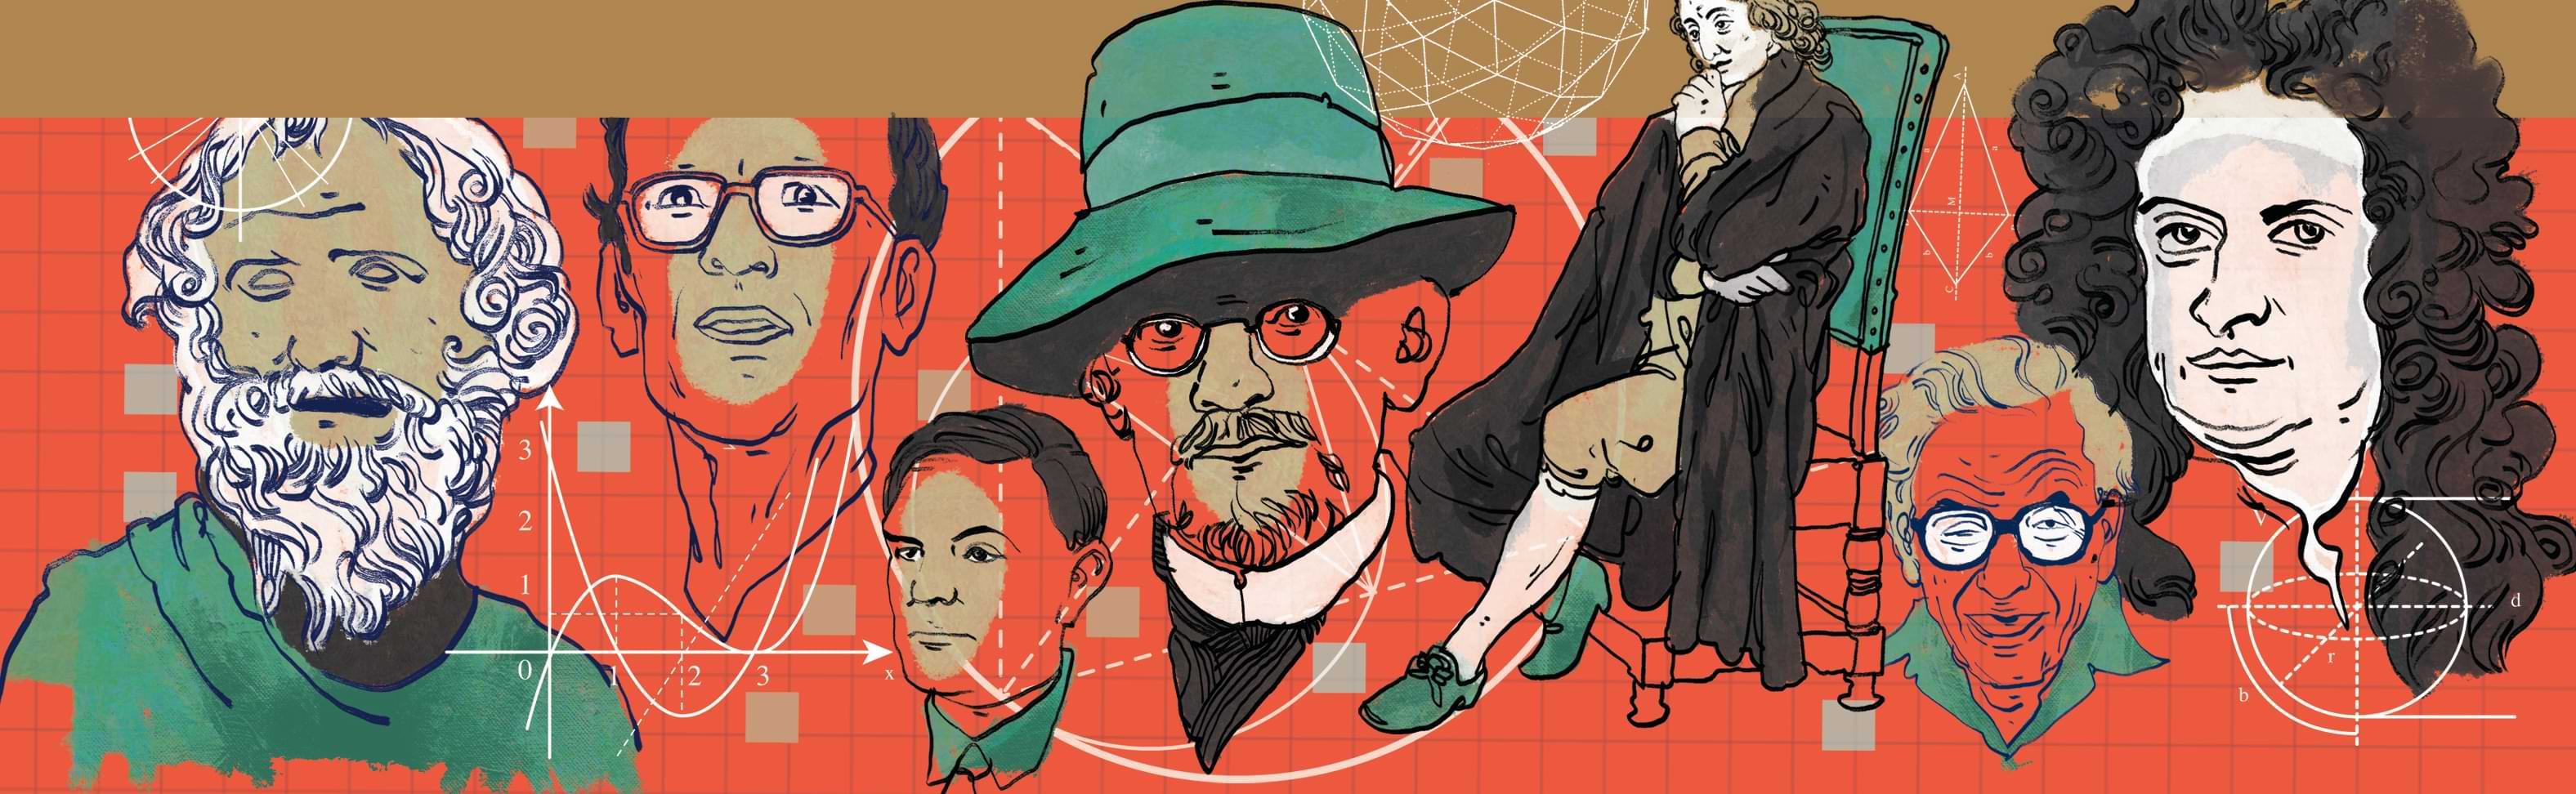
\includegraphics[width=19.3cm]{../bannerlichsu}}}
\AddToShipoutPicture*{\put(58,469){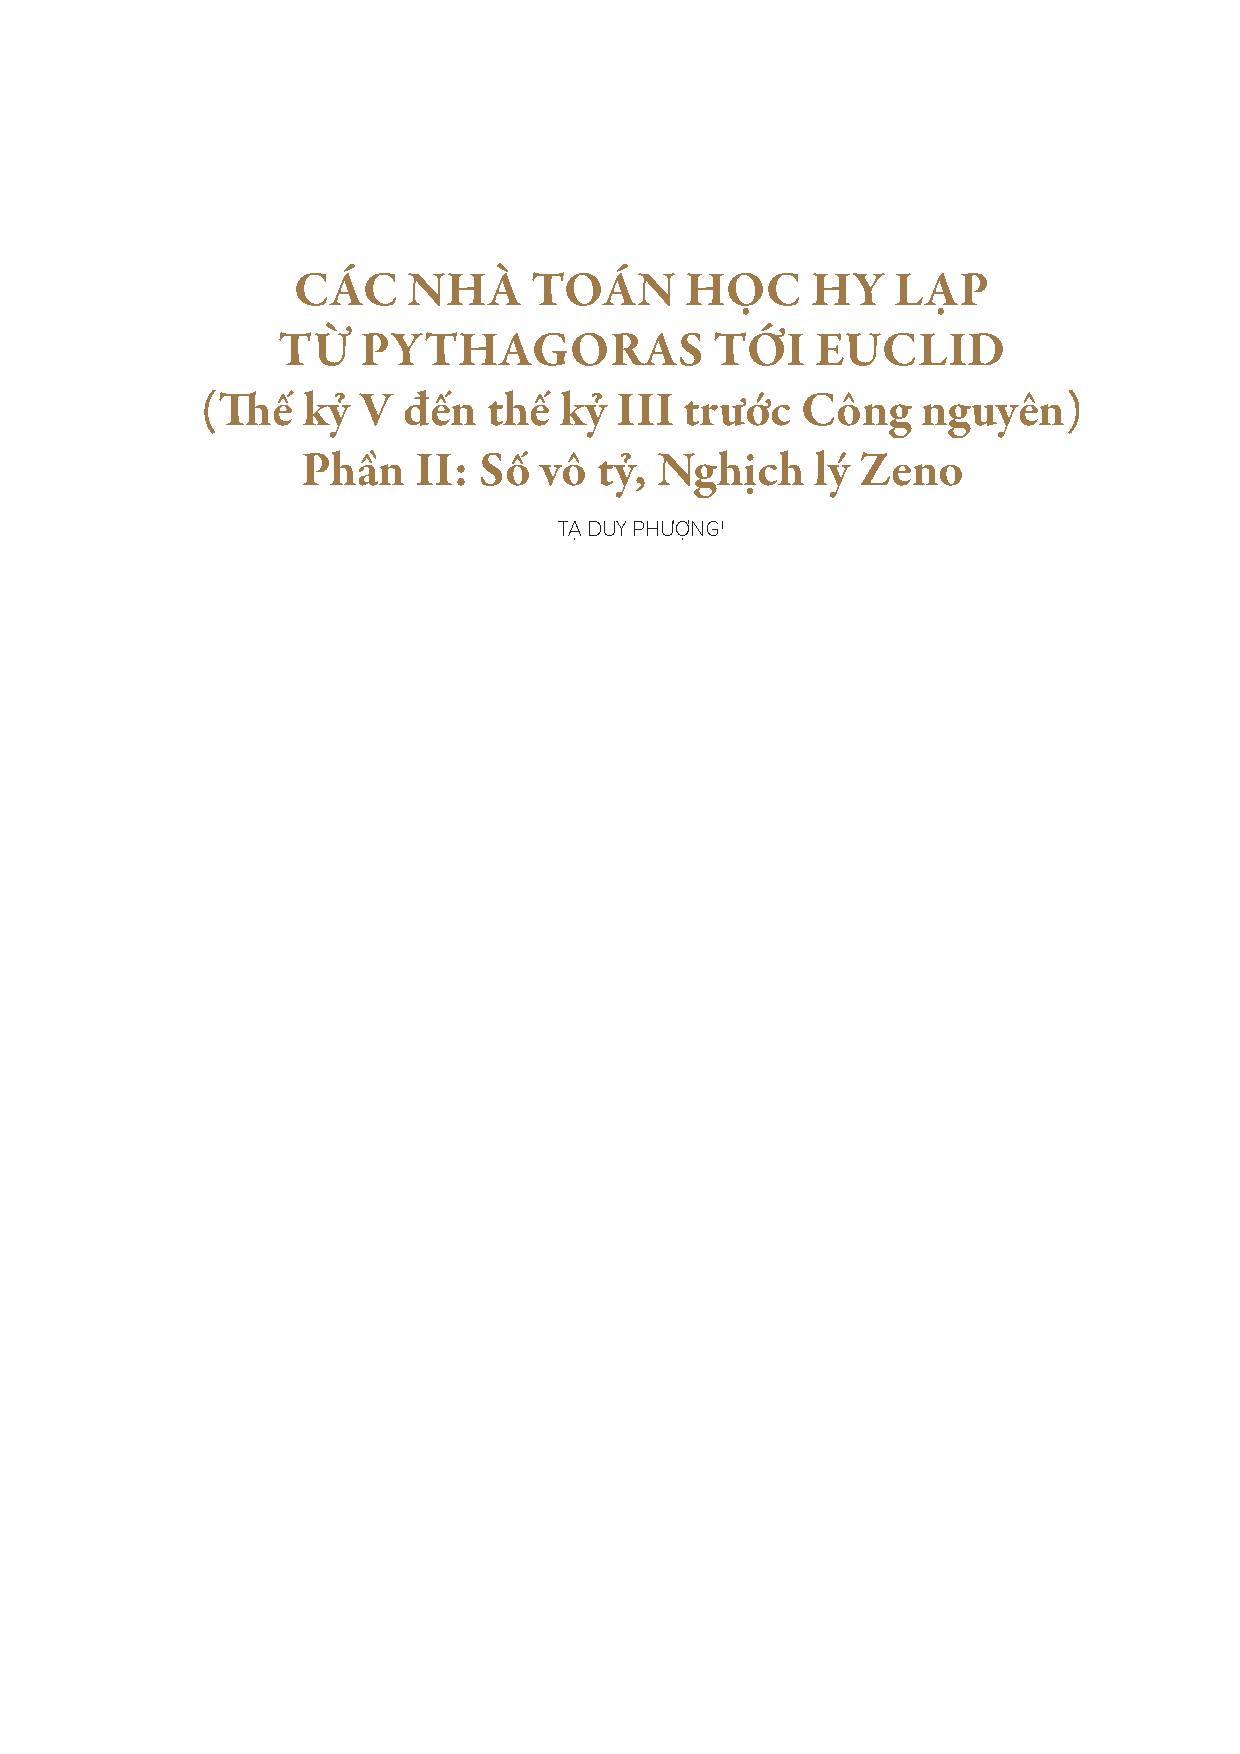
\includegraphics[scale=1]{../tieude.pdf}}}
\centering
\endgroup

\vspace*{235pt}

\begin{multicols}{2}
%	\setlength{\abovedisplayskip}{5pt}
%	\setlength{\belowdisplayskip}{5pt}
	$\pmb{1.}$ \textbf{\color{lichsutoanhoc}Số vô tỷ}
	\vskip 0.05cm
	Hippasus xứ Croton, khoảng $530-450$ trước công nguyên (TCN), ban đầu là người thuộc trường phái Pythagoras, nhưng sau bị khai trừ khỏi trường phái này. Một tài liệu nói những người Pythagoras đã dựng bia mộ ông, như thể ông đã chết; một tài liệu khác nói rằng sự bội đạo của ông đã bị trừng phạt bằng cái chết trên biển trong một tai nạn chìm tàu. Nguyên nhân chính xác có lẽ không bao giờ được biết, do quy tắc bí mật của trường phái Pythagoras, nhưng có ba khả năng đã được nêu ra. 
	\vskip 0.05cm
	Khả năng thứ nhất, Hippasus bị trục xuất vì ông đứng đầu một phong trào dân chủ chống lại những quy định bảo thủ của Pythagoras.
	\vskip 0.05cm
	Khả năng thứ hai quy việc trục xuất ông về lý do ông đã tiết lộ các phát minh của trường phái Pythagoras về ngũ giác đều hoặc khối $12$ mặt đều. 
	\vskip 0.05cm
	Giải thích thứ ba cho rằng ông bị trục xuất vì tiết lộ một khám phá toán học có ý nghĩa tàn khốc đối với học thuyết Pythagoras -- sự tồn tại các số vô tỷ.
	\vskip 0.1cm
	Nguyên lý cơ bản của học thuyết Pythagoras là các thuộc tính của số nguyên hoặc tỷ lệ của chúng (các số hữu tỷ) có thể giải thích bản chất của tất cả mọi thứ, trong hình học cũng như trong thiên văn và xã hội. Tuy nhiên, \textit{Đối thoại} của Plato (khoảng $428-347$ TCN) cho thấy rằng cộng đồng toán học Hy Lạp đã bị choáng váng bởi một tiết lộ hầu như phá hủy toàn bộ niềm tin của người Pythagoras và cộng đồng vào những con số. Đây là khám phá rằng trong bản  thân hình học, các số hữu tỷ không đủ để giải thích các thuộc tính cơ bản. Chẳng hạn, số hữu tỷ không đủ để so sánh tỷ lệ của đường chéo hình vuông, đường chéo hình lập phương hoặc đường chéo ngũ giác đều với cạnh của~nó. 
	\vskip 0.1cm
	Thông thường, người ta cho rằng sự công nhận số vô tỷ liên quan đến ứng dụng của định lý Pythagoras vào tam giác vuông cân. Một chứng minh như vậy rất dễ xây dựng (xem [$10$]). Aristotle ($384-322$ TCN) đã đề cập đến một chứng minh về tính không thông ước$^{\small2}$ của đường chéo của hình vuông với cạnh của nó. Trong chứng minh này, mức độ trừu tượng cao đến mức người ta nghi ngờ nó đã được thực hiện vào thế kỷ V TCN. Tuy nhiên,  khám phá về số vô tỷ có thể đã xảy ra vào thế kỷ V TCN theo những cách khác. 
	\vskip 0.1cm
	\blfootnote{\color{lichsutoanhoc}$^2$Hai đoạn thẳng có độ dài $a$ và $b$ được gọi là thông ước với nhau nếu tồn tại một đoạn thẳng có độ dài $c$ và các số tự nhiên $m$ và $n$ sao cho $a = mc$ và $b = nc$, tức là $\frac{a}{b} = \frac{m}{n}$. Theo ngôn ngữ ngày nay, hai đại lượng là thông ước nếu thương của chúng là một số hữu tỷ.}
	Năm đường chéo của một ngũ giác đều tạo thành một ngũ giác đều nhỏ hơn và các đường chéo của hình ngũ giác thứ hai lần lượt tạo thành hình ngũ giác đều thứ ba ... (Hình $1$).
	\begin{figure}[H]
		\vspace*{-10pt}
		\centering
		\captionsetup{labelformat= empty, justification=centering}
		\begin{tikzpicture}[lichsutoanhoc,scale=0.75]
			\draw  (-1.,1.)-- (2.,1.);
			\draw  (2.,1.)-- (2.9270509831248424,3.85316954888546);
			\draw  (2.9270509831248424,3.85316954888546)-- (0.5,5.616525305762879);
			\draw  (0.5,5.616525305762879)-- (-1.927050983124842,3.853169548885461);
			\draw  (-1.927050983124842,3.853169548885461)-- (-1.,1.);
			\draw  (0.5,5.616525305762879)-- (2.,1.);
			\draw  (0.5,5.616525305762879)-- (-1.,1.);
			\draw  (-1.927050983124842,3.853169548885461)-- (2.9270509831248424,3.85316954888546);
			\draw  (2.9270509831248424,3.85316954888546)-- (-1.,1.);
			\draw  (-1.927050983124842,3.853169548885461)-- (2.,1.);
			\draw  (-0.07294901687515731,3.85316954888546)-- (1.4270509831248426,2.763355756877419);
			\draw  (-0.07294901687515731,3.85316954888546)-- (0.5,2.0898137920080413);
			\draw  (0.5,2.0898137920080413)-- (1.0729490168751583,3.853169548885459);
			\draw  (1.0729490168751583,3.853169548885459)-- (-0.4270509831248419,2.763355756877419);
			\draw  (-0.4270509831248419,2.763355756877419)-- (1.4270509831248426,2.763355756877419);
		\end{tikzpicture}
		\caption{\small\textit{\color{lichsutoanhoc}Hình $1$.}}
		\vspace*{-10pt}
	\end{figure}
	Quá trình này có thể được tiếp tục đến vô hạn, dẫn đến gợi ý: \textit{Tỷ số giữa một đường chéo và một cạnh của một ngũ giác đều không thể là số hữu tỷ.} 
	\vskip 0.1cm
	Xét ngũ giác đều $ABCDE$  với hai đường chéo $AD$  và $BE$  (Hình $2$). Do $\angle ABE = \angle IAE$ và $\angle AEB = \angle IEA$  nên $\Delta ABE \sim \Delta IAE$.  
	\begin{figure}[H]
		\vspace*{-10pt}
		\centering
		\captionsetup{labelformat= empty, justification=centering}
		\begin{tikzpicture}[lichsutoanhoc,scale=0.75]
			\draw  (1.5,4.616525305762879)-- (3.9270509831248424,2.85316954888546);
			\draw  (3.9270509831248424,2.85316954888546)-- (3.,0.);
			\draw  (3.,0.)-- (0.,0.);
			\draw  (0.,0.)-- (-0.9270509831248419,2.853169548885461);
			\draw  (-0.9270509831248419,2.853169548885461)-- (1.5,4.616525305762879);
			\draw  (-0.9270509831248419,2.853169548885461)-- (3.9270509831248424,2.85316954888546);
			\draw  (1.5,4.616525305762879)-- (0.,0.);
	
				\draw [fill=white] (0.,0.) circle (1.5pt);
				\draw (-0.24,-0.23) node {$D$};
				\draw [fill=white] (3.,0.) circle (1.5pt);
				\draw (3.16,-0.23) node {$C$};
				\draw [fill=white] (3.9270509831248424,2.85316954888546) circle (1.5pt);
				\draw (4.06,3.23) node {$B$};
				\draw [fill=white] (1.5,4.616525305762879) circle (1.5pt);
				\draw (1.64,4.99) node {$A$};
				\draw [fill=white] (-0.9270509831248419,2.853169548885461) circle (1.5pt);
				\draw (-1.1,3.29) node {$E$};
				\draw [fill=white] (0.9270509831248427,2.8531695488854605) circle (1.5pt);
				\draw (0.82,3.19) node {$I$};
		\end{tikzpicture}
		\caption{\small\textit{\color{lichsutoanhoc}Hình $2$.}}
		\vspace*{-10pt}
	\end{figure}
	Suy ra $\dfrac{AB}{BE} = \dfrac{IA}{AE}$. Nhưng $AE = AB$  nên 
	\begin{align*}
		&A{B^2} = BE \times IA = BE \times \left( {BE - AB} \right)\\
		\Rightarrow \,& A{B^2} = B{E^2} - BE \times AB.
	\end{align*}
	Chia cả hai vế cho $AB^2$  và đặt $\dfrac{BE}{AB} = x$  ta được $x^2 - x - 1= 0$.  Suy ra $\dfrac{BE}{AB} = x = \dfrac{1 + \sqrt{5}}{2}$. Suy ra $\dfrac{AB}{BE} = \dfrac{1}{x} = \dfrac{\sqrt{5} -1}{2}$. Số $x = \dfrac{1 + \sqrt{5}}{2}$  hoặc $\dfrac{1}{x} = \dfrac{\sqrt{5} - 1}{2}$  được gọi là \textit{tỷ lệ vàng}.
	\vskip 0.1cm
	Có vẻ như, không phải là $\sqrt{2}$  mà là  $\sqrt{5}$ lần đầu tiên tiết lộ sự tồn tại của các số vô tỷ (thông qua các đại lượng không thông ước đến từ ngũ giác đều). Tính chất vô tỷ của tỷ lệ này, trên thực tế, là hệ quả của lập luận được trình bày trên Hình $3$, trong đó tỷ lệ vàng được hiển thị lặp đi lặp lại nhiều lần:
	\begin{align*}
		\frac{{R{P_1}}}{{{P_1}S}} = \frac{{R{P_2}}}{{{P_2}{P_1}}} = \frac{{R{P_3}}}{{{P_3}{P_2}}} = \ldots
	\end{align*}
	\begin{figure}[H]
		\vspace*{-10pt}
		\centering
		\captionsetup{labelformat= empty, justification=centering}
		\begin{tikzpicture}[lichsutoanhoc,scale=0.68]
			\draw  (0.,0.)-- (10.,0.);
				\draw  (0.,0.) -- (0,0.2);
				\draw (0.0,-0.5) node {$R$};
				\draw  (10,0.) -- (10,0.2);
				\draw (10,-0.5) node {$S$};
				\draw  (6.2,0.) -- (6.2,0.2);
				\draw (6.2,-0.5) node {$P_1$};
				\draw  (3.8,0.) -- (3.8,0.2);
				\draw (3.8,-0.5) node {$P_2$};
				\draw  (2.4,0.) -- (2.4,0.2);
				\draw (2.4,-0.5) node {$P_3$};
		\end{tikzpicture}
		\caption{\small\textit{\color{lichsutoanhoc}Hình $3$.}}
		\vspace*{-10pt}
	\end{figure}
	Tính chất này dẫn đến việc tiết lộ, có thể bởi Hippasus, về tính không thông ước giữa đường chéo của ngũ giác đều và cạnh của nó. Không có tài liệu nào khẳng định điều này, nhưng có vẻ như đây là một suy đoán có lý.
	\vskip 0.1cm
	Tỷ lệ giữa đường chéo của hình lập phương với một cạnh bằng $\sqrt{3}$, cũng dẫn tới tính không thông ước của đường chéo và cạnh của hình lập phương, hay tính chất vô tỷ của số $\sqrt{3}$.
	\begin{figure}[H]
		\vspace*{-10pt}
		\centering
		\captionsetup{labelformat= empty, justification=centering}
		\begin{tikzpicture}[lichsutoanhoc,scale=0.8]
			\draw  (0.,0.)-- (4.,0.);
			\draw  (4.,0.)-- (4.,4.);
			\draw  (4.,4.)-- (0.,4.);
			\draw  (0.,4.)-- (0.,0.);
			\draw  (4.,4.)-- (0.,0.);
			\draw  (3.31370849898476,4.)-- (3.3137084989847594,3.3137084989847585);
			\draw  (1.6568542494923808,4.)-- (2.8284271247461903,2.82842712474619);
			
			\draw [fill=white] (0.,0.) circle (1.5pt);
			\draw (-0.2,-0.17) node {$A$};
			\draw [fill=white] (4.,0.) circle (1.5pt);
			\draw (4.22,-0.13) node {$D$};
			\draw [fill=white] (4.,4.) circle (1.5pt);
			\draw (4.16,4.41) node {$C$};
			\draw [fill=white] (0.,4.) circle (1.5pt);
			\draw (-0.16,4.35) node {$B$};
			\draw [fill=white] (1.6568542494923808,4.) circle (1.5pt);
			\draw (1.62,4.41) node {$Q$};
			\draw [fill=white] (3.31370849898476,4.) circle (1.5pt);
			\draw (3.28,4.41) node {$R$};
			\draw [fill=white] (3.31370849898476,4.) circle (1.5pt);
			\draw [fill=white] (3.3137084989847594,3.3137084989847585) circle (1.5pt);
			\draw (3.56,3.05) node {$S$};
			\draw [fill=white] (2.8284271247461903,2.82842712474619) circle (1.5pt);
			\draw (2.86,2.51) node {$P$};
		\end{tikzpicture}
		\caption{\small\textit{\color{lichsutoanhoc}Hình $4$.}}
		\vspace*{-5pt}
	\end{figure}
	Tương tự như ngũ giác đều, nếu trong hình vuông $ABCD$ (Hình $4$) dựng trên đường chéo $AC$ đoạn $AP = AB$  và tại $P$ dựng đoạn thẳng $PQ$  vuông góc với đường chéo thì $\dfrac{CQ}{CP} = \dfrac{AC}{AB}$. Một lần nữa, nếu trên $CQ$  đặt $QR = QP$ và  dựng $RS$  vuông góc với $CR$,  thì  $\dfrac{CS}{CR} = \dfrac{CQ}{CP} = \dfrac{AC}{AB}$. Quá trình này có thể được lặp lại vô hạn. Đây một chứng minh cho thấy không có đơn vị độ dài nào, dù nhỏ, có thể được tìm thấy để đường chéo và cạnh hình vuông là thông ước với nhau.
	\vskip 0.1cm
	\PIbox{\textbf{\color{lichsutoanhoc}Bài tập.} Sử dụng chứng minh $\sqrt{2}$  là số vô tỷ (xem [$10$]), hãy chứng minh $\sqrt{3}$  là số vô tỷ, hay đường chéo của hình lập phương không thông ước với cạnh của nó. Tương tự, chứng minh $\sqrt{5}$ là số vô tỷ.}
	\vskip 0.1cm
	$\pmb{2.}$ \textbf{\color{lichsutoanhoc}Nghịch lý Zeno}
	\vskip 0.1cm
	Học thuyết Pythagoras cho rằng ``Các con số [hữu tỷ] tạo nên toàn bộ thiên đường" thực sự đã phải đối mặt với một vấn đề rất nghiêm trọng khi số vô tỷ được phát hiện, nhưng trường phái Pythagoras còn phải đối mặt với những lập luận do những học giả xứ Elea, một trường phái đối thủ đưa ra. 
	\vskip 0.1cm
	Các nhà triết học Ionia ở Tiểu Á đã tìm cách xác định yếu tố cơ bản của vật chất.
	\vskip 0.1cm
	Thales cho rằng nước là nguồn gốc của vật chất, nhưng những người khác ưu tiên coi không khí hoặc lửa là yếu tố cơ bản. Trường phái Pythagoras đã theo một hướng trừu tượng hơn: cho rằng các con số (hữu tỷ) là cơ bản. Thuyết này, được minh họa một cách tuyệt đẹp trong hình học của các con số tượng hình, đã bị công kích bởi những người theo Parmenides (đầu thế kỷ V TCN) xứ Elea. Nguyên lý cơ bản của trường phái Elea là sự thống nhất và vĩnh viễn, một quan điểm trái ngược với các ý tưởng của Pythagoras về tính đa dạng và thay đổi.  Trong các môn đệ của Parmenides, người được biết đến nhiều nhất là Zeno ở Elea (khoảng $495-430$ TCN), người đã đưa ra các lý lẽ để chứng minh sự mâu thuẫn trong các khái niệm của Pythagoras.
	\vskip 0.1cm
	Những người Pythagoras cho rằng không gian và thời gian có thể được coi là bao gồm các điểm và cá thể, nhưng không gian và thời gian cũng có thuộc tính, được gọi là ``tính liên tục". 
	Một mặt, tính liên tục có các đặc điểm của đơn vị hình học -- điểm -- và mặt khác, có các đặc điểm của các đơn vị số hoặc các số.
	Aristotle ($384-322$ TCN) đã mô tả quan điểm của Pythagoras là ``sự thống nhất có vị trí" hoặc ``sự thống nhất được xem xét trong không gian". 
	Để chống lại quan điểm này, Zeno đưa ra những nghịch lý, trong đó các nghịch lý về chuyển động dường như đã gây ra nhiều rắc rối nhất:
	\vskip 0.1cm
	$(1)$ Sự phân đôi (the Dichotomy), 
	\vskip 0.1cm
	$(2)$ Achilles và con rùa, 
	\vskip 0.1cm
	$(3)$ Mũi tên (the Arrow), và 
	\vskip 0.1cm
	$(4)$ Sân vận động (the Stade, hay Stadium).
	\vskip 0.1cm
	\textbf{\color{lichsutoanhoc}Sự phân đôi}
	\vskip 0.1cm
	Một người chạy được một quãng đường nhất định, trước tiên anh ta phải đi một nửa quãng đường này, nhưng trước khi anh ta có thể làm được điều này, anh ta phải đi một phần tư quãng đường đầu tiên, và trước đó, một phần tám quãng đường đầu tiên, và cứ như vậy, thông qua vô số đoạn.  Anh ta phải tạo vô số đoạn trong một thời gian hữu hạn, nhưng điều này là không thể. Do đó sự khởi động của chuyển động là không thể.
	\vskip 0.1cm
	\textbf{\color{lichsutoanhoc}Achilles và con rùa}
	\vskip 0.1cm
	Nghịch lý thứ hai tương tự như nghịch lý thứ nhất, ngoại trừ việc chia nhỏ vô hạn không gian là lũy tiến, chứ không phải là thoái lui. Giả sử Achilles chạy đua với một con rùa đã xuất phát từ trước. Khi Achilles đạt đến vị trí ban đầu của con rùa, thì con rùa đã đi được một đoạn ngắn và vào thời điểm Achilles vượt qua đoạn này, con rùa sẽ tiến lên hơi xa hơn, và quá trình này tiếp tục vô hạn, với kết quả là Achilles nhanh nhẹn không bao giờ có thể vượt qua con rùa chậm chạp.
	\vskip 0.1cm
	\textbf{\color{lichsutoanhoc}Mũi tên}
	\vskip 0.05cm
	Các nghịch lý \textit{Phân đôi} và \textit{Achilles} lập luận rằng chuyển động là không thể dưới giả thiết về sự chia nhỏ vô hạn không gian và thời gian. Mặt khác, \textit{Mũi tên} và \textit{Sân vận động} lập luận rằng chuyển động không thể xảy ra nếu giả định ngược lại rằng có một đại lượng nhỏ nhất của không gian và thời gian. Trong \textit{Mũi tên}, Zeno lập luận rằng một vật thể đang bay vào mỗi khoảnh khắc cũng chiếm một khoảng không gian bằng chính nó. Như vậy trong khoảnh khắc đó nó không chuyển động. Vì thế mũi tên đang bay luôn dừng, do đó chuyển động của nó chỉ là một ảo giác.
	\vskip 0.05cm
	\textbf{\color{lichsutoanhoc}Sân vận động}
	\vskip 0.05cm
	Gây tranh cãi nhiều nhất và khó xử nhất về những nghịch lý trong chuyển động là \textit{Sân vận động}, nó có thể được diễn giải như sau. 
	\vskip 0.1cm
	Giả sử rằng tại một thời điểm nhất định, các vật ${A_1}$, ${A_2}$, ${A_3}$, ${A_4}$, ${A_5}$, ${A_6}$, $A_7$, $A_8$; $B_1$, $B_2$, $B_3$, $B_4$, $B_5$, $B_6$, $B_7$, $B_8$  và $C_1$, $C_3$, $C_3,$ $C_4$, $C_5$, $C_6$, $C_7$, $C_8$ chiếm các vị trí tương đối sau \linebreak(Hình $5a$):
	\begin{figure}[H]
		\vspace*{-10pt}
		\centering
		\captionsetup{labelformat= empty, justification=centering}
		\begin{tikzpicture}[scale=0.44,lichsutoanhoc,node font=\scriptsize]
			\draw (0,0) grid (8,1);
			\draw (0,2) grid (-8,3);
			\draw (-4,4) grid (4,5);
			\draw[-stealth] (-1,0.5) -- (-3, 0.5);
			\draw[-stealth] (1,2.5) -- (3, 2.5);

			\foreach \x in {1,2,...,8}{
				\node at (\x-0.5, 0.5) {$C_\x$};
				\node at (\x - 4.5, 4.5) {$A_\x$};
				\node at (-\x + 0.5, 2.5) {$B_\x$};}
		\end{tikzpicture}
		\caption{\small\textit{\color{lichsutoanhoc}Hình $5a$: Sân vận động.}}
		\vspace*{-10pt}
	\end{figure}
	Các vật $B$ chuyển động sang phải và các vật $C$ chuyển động sang trái với cùng vận tốc để được Hình $5b$:
	\begin{figure}[H]
	\vspace*{-10pt}
	\centering
	\captionsetup{labelformat= empty, justification=centering}
	\begin{tikzpicture}[scale=0.45,lichsutoanhoc,node font=\scriptsize]
		\draw (0,0) grid (8,1);
		\draw (0,2) grid (8,3);
		\draw (0,4) grid (8,5);
		
		\foreach \x in {1,2,...,8}{
			\node at (\x-0.5, 0.5) {$C_\x$};
			\node at (\x-0.5, 4.5) {$A_\x$};
			\node at (8.5-\x, 2.5) {$B_\x$};}
	\end{tikzpicture}
	\caption{\small\textit{\color{lichsutoanhoc}Hình $5b$: Sân vận động.}}
	\vspace*{-5pt}
	\end{figure}
	Khi $C_1$  đi qua $8$ vật $B$  (và $B_1$ đi qua 8 vật  $C$) thì $B_1$  chỉ đi qua $4$ vật $A_5, A_6, A_7, A_8$  (tương tự,  $C_1$  đi qua $4$ vật  $A_1, A_2, A_3, A_4$). Nhưng $C_1$  mất cùng một thời gian khi đi qua $8$ vật  $B$ như là đi qua $4$ vật $A$.  Suy ra thời gian để  $C_1$  đi qua $8$ vật $A$  cũng bằng thời gian đi qua một nửa $A$,  hay thời gian đã cho bằng một nửa của nó. Mâu thuẫn.     
	\vskip 0.1cm
	Aristotle cho rằng Zeno đã không hiểu sự khác nhau giữa chuyển động tương đối với chuyển động tuyệt đối và tin rằng ông đã bác bỏ nghịch lý của Zeno vì ông đã phủ nhận giả định ban đầu: thời gian bao gồm các đơn vị không thể phân chia. Tuy nhiên, giải thích thấu đáo nghịch lý Zeno về sân vận động chỉ được đưa ra bởi Brochard, Noël và Russell vào thế kỷ XIX--XX.
	\vskip 0.1cm 
	Các lập luận của Zeno dường như đã có ảnh hưởng sâu sắc đến sự phát triển của toán học Hy Lạp, có thể so sánh với sự phát hiện ra số vô tỷ, mà chúng có thể có liên quan với nhau. Ban đầu, trong lý thuyết của Pythagoras, độ lớn được biểu thị bằng hạt hoặc đá cuội, nhưng đến thời Euclid thì có một sự thay đổi hoàn toàn về quan điểm.  Độ lớn nói chung không phải được liên kết với các con số hoặc viên sỏi, mà với các đoạn thẳng. Trong \textit{Cơ sở}, thậm chí các số nguyên cũng được biểu diễn bằng các đoạn. Vương quốc của con số có đặc tính rời rạc, nhưng thế giới của các đại lượng liên tục là một thứ ngoài số và phải được xử lý bằng phương pháp hình học (và điều này bao gồm hầu hết toán học thời kỳ tiền cổ đại và Pythagoras).  Dường như là hình học, hơn là con số, thống trị thế giới.
	\vskip 0.1cm
	\textbf{\color{lichsutoanhoc}Tài liệu trích dẫn}
	\vskip 0.1cm
	[$10$] Tạ Duy Phượng, \textit{Pythagoras và trường phái toán học Pythagoras}, Tạp chí Pi, Tập $6$ ($2022$), số $5$, trang $45-53$.
\end{multicols}